\documentclass[10pt,twocolumn]{article}

% ─── Packages ────────────────────────────────────────────────────────────────
\usepackage[margin=0.75in,top=1in,bottom=1in]{geometry}
\usepackage[T1]{fontenc}
\renewcommand{\rmdefault}{ptm}
\usepackage{amsmath}
\usepackage{amssymb}
\usepackage{graphicx}
\usepackage{booktabs}
\usepackage{hyperref}
\usepackage{url}
\usepackage[numbers,sort&compress]{natbib}
\usepackage{xcolor}
\usepackage{microtype}
\usepackage{caption}
\usepackage{subcaption}
\usepackage{tikz}
\usetikzlibrary{shapes.geometric, arrows.meta, positioning, fit, backgrounds}
\usepackage{float}

\hypersetup{
    colorlinks=true,
    linkcolor=blue,
    citecolor=blue,
    urlcolor=blue
}

\setlength{\columnsep}{0.25in}
\raggedbottom

% ─── Tighter section spacing ──────────────────────────────────────────────────
\makeatletter
\renewcommand\section{\@startsection{section}{1}{\z@}%
  {-2.3ex \@plus -1ex \@minus -.2ex}%
  {1ex \@plus .2ex}%
  {\normalfont\Large\bfseries}}
\renewcommand\subsection{\@startsection{subsection}{2}{\z@}%
  {-2ex\@plus -1ex \@minus -.2ex}%
  {0.75ex \@plus .2ex}%
  {\normalfont\large\bfseries}}
\renewcommand\subsubsection{\@startsection{subsubsection}{3}{\z@}%
  {-1.8ex\@plus -1ex \@minus -.2ex}%
  {0.5ex \@plus .2ex}%
  {\normalfont\normalsize\bfseries}}
\makeatother

% ─── Title ───────────────────────────────────────────────────────────────────
\title{
    \Large\textbf{Benchmarking Sensor Robustness in Plasma Diagnostic Models:}\\
    \Large\textbf{A Systematic Evaluation on TokaMark}
}

\author{
    Neerav Gupta \\
    \small Independent Researcher \\
    \small \texttt{neerav.dgupta@gmail.com}
}

\date{}

% ─────────────────────────────────────────────────────────────────────────────
\begin{document}
\maketitle

% ─── Abstract ────────────────────────────────────────────────────────────────
\begin{abstract}
Plasma diagnostic models for tokamak fusion devices are almost universally
evaluated on clean, complete sensor data. In practice, however, fusion
diagnostics fail regularly—acquisition systems start late, individual
sensors die, and signal dropouts cluster precisely when a plasma disruption
is approaching. We present the first systematic robustness benchmark for
plasma diagnostic ML using the TokaMark dataset of 11,573 MAST
shots~\cite{rousseau2026tokamark}, evaluating XGBoost, LSTM, and
Transformer models across six physically-grounded failure scenarios and
three imputation strategies. We also introduce the Robustness Score (RS),
a standardized cross-architecture metric. Our central finding is that
disruption-proximate sensor failure—corruption injected in the final
window timesteps—collapses sequence model performance (LSTM $+212\%$
NRMSE) while a statistical feature model remains comparatively stable
(XGBoost $+37\%$). Forward-fill imputation eliminates nearly all
degradation from random dropout for sequence models (LSTM $+57\% \to
{\sim}0\%$), but offers little help when the end of the window is
corrupted. Plasma current emerges as the single most critical diagnostic
across all architectures ($+73\%$ to $+140\%$ upon removal). Notably,
front-loaded acquisition gaps—the most common natural failure pattern
in MAST—leave model performance essentially unchanged.
Code, data, and trained checkpoints are available at
\url{https://github.com/Neerav-Gupta/tokamark-robustness}.
\end{abstract}

% ─── 1. Introduction ─────────────────────────────────────────────────────────
\section{Introduction}

\subsection{Nuclear Fusion and Tokamaks}

Nuclear fusion has long been considered one of the most compelling
paths toward clean, abundant energy. Where fission splits heavy atoms
and leaves behind radioactive byproducts, fusion joins light hydrogen
isotopes—deuterium and tritium—and releases substantially more
energy per reaction, with helium as the main product~\cite{freidberg2007}.
The fuel supply is effectively inexhaustible: deuterium is extracted
from seawater, and tritium can be bred from lithium. A working fusion
power plant would emit no carbon, produce no long-lived radioactive
waste, and carry no risk of a runaway reaction~\cite{wesson2004}.

The central difficulty is confining the fuel long enough for fusion to
occur. The reaction requires temperatures above 100 million degrees
Celsius—hotter than the core of the Sun—at which hydrogen exists
as a plasma that would instantly destroy any material it contacted.
Magnetic confinement fusion (MCF) handles this by using carefully shaped
magnetic fields to keep the plasma suspended away from reactor
walls~\cite{freidberg2007}. Among MCF concepts, the tokamak has proven
the most successful, and ITER—now under construction in southern
France at an estimated cost of \$22 billion—is the international
experiment intended to demonstrate net energy gain from fusion for the
first time~\cite{iter1999}.

\subsection{Disruptions: The Critical Safety Challenge}

A plasma disruption is a sudden, uncontrolled loss of plasma confinement:
within milliseconds, the thermal and magnetic energy stored in the plasma
dumps into the reactor walls~\cite{devries2011}. De~Vries et
al.~\cite{devries2011} catalogued disruptions at JET—the Joint European
Torus and the world's largest operating tokamak—finding they occur in
roughly 3--4\% of routine plasma shots, with higher rates under demanding
operating conditions. At the scale of ITER or a commercial plant, each
disruption inflicts heat loads, electromagnetic impulses, and runaway
electron beams capable of permanently damaging the first wall, magnets,
and structural components~\cite{iter1999}.

The economic stakes are considerable. Maris et al.~\cite{maris2024}
showed that even moderate disruption rates push up the levelized cost
of electricity enough to threaten the commercial viability of fusion
energy. The practical response is early disruption prediction: if a
machine's control system receives even 50--100 milliseconds of warning,
it can gracefully terminate the plasma before damage
occurs~\cite{katesharbeck2019}. Reliable, real-time prediction is
therefore not merely a performance goal—it is a safety requirement
for any reactor-class device.

\subsection{AI for Plasma Prediction}

Plasma physics is complex and the diagnostic environment is demanding,
which together create a strong case for data-driven methods. Fusion
diagnostics cover magnetics, optical emission, X-ray cameras, microwave
interferometry, and more, spanning sampling rates from 200 Hz to 500 kHz
and producing inherently multi-modal, asynchronous, and noisy
data~\cite{morris2002}. Machine learning models can fuse these
heterogeneous streams, respond in real time, and capture nonlinear
dynamics without requiring explicit physical parameterization~\cite{churchill2025}.

Progress has been rapid. Kates-Harbeck et al.~\cite{katesharbeck2019}
showed that deep recurrent networks trained on raw diagnostic time series
could predict disruptions across JET and DIII-D with strong performance.
Vega et al.~\cite{vega2022} took this further, deploying an AI-based
disruption prediction system at JET that matched or outperformed existing
physics-based predictors. Churchill et al.~\cite{churchill2020} demonstrated
that convolutional networks operating directly on high-resolution
diagnostics could reliably identify pre-disruption states on DIII-D.
More recently, foundation model approaches have been proposed as a
path toward general-purpose plasma representations: Churchill~\cite{churchill2025}
laid out the theoretical case, and TokaMind~\cite{boschi2026tokamind}
delivered the first open-source multi-modal transformer trained on MAST
data and benchmarked on TokaMark tasks.

\subsection{The Missing Robustness Problem}

Despite this progress, almost every published evaluation rests on the
same unstated assumption: that sensor data arriving at inference time
is complete and clean. In practice this assumption regularly fails.
Acquisition systems start late, producing front-loaded gaps that cover
10--16\% of signal history. Individual sensors fail mid-shot due to
heat damage and electromagnetic interference. And these failures are
not uniformly distributed in time—they tend to occur precisely when
the plasma is most unstable and prediction is most critical. A
disruption produces intense heat loads and electromagnetic transients
that actively degrade sensor performance in the moments leading up to
the event~\cite{rousseau2026tokamark, jackson2025ieee}.

TokaMark~\cite{rousseau2026tokamark} acknowledges this directly,
identifying robustness to incomplete state information as one of its
four core benchmark dimensions and noting that signals ``may be absent
for a given shot due to hardware issues'' or ``contain missing time
segments due to limited acquisition windows or diagnostic failures.''
Yet no evaluation of this dimension appears anywhere in the TokaMark
paper, and no prior work has systematically studied how plasma
diagnostic models degrade under controlled sensor failure.

This paper addresses that gap directly. Our contributions are:

\begin{enumerate}
    \renewcommand{\labelenumi}{(\arabic{enumi})}
    \item \textbf{Natural missingness characterization.} We stream
    300 MAST shots from FAIR-MAST and characterize the real NaN
    structure of each diagnostic category, finding that failures
    are front-loaded and category-correlated—directly informing
    our scenario design.

    \item \textbf{Six physically-grounded failure scenarios.} We
    implement random dropout, channel ablation, temporal gaps (front,
    random, pre-event), correlated diagnostic group failure, and
    disruption-proximate failure. The last scenario, to our knowledge,
    has not been evaluated in any prior work.

    \item \textbf{Cross-architecture robustness benchmark.} We evaluate
    XGBoost, LSTM, and Transformer on Task~4-4 under all six scenarios,
    and introduce the Robustness Score (RS) as a standardized metric
    we encourage the community to adopt.

    \item \textbf{Mitigation strategy evaluation.} We evaluate zero-fill,
    mean-fill, and forward-fill imputation across all scenarios,
    establishing which strategies work, which do not, and why.
\end{enumerate}

% ─── 2. Related Work ─────────────────────────────────────────────────────────
\section{Related Work}

\paragraph{TokaMark and FAIR-MAST.}
Rousseau et al.~\cite{rousseau2026tokamark} introduced TokaMark as the
first large-scale, openly available benchmark for AI models on real
fusion data, defining 14 tasks across four groups over an 80/10/10
shot-level split drawn from the FAIR-MAST
dataset~\cite{jackson2024softwarex, jackson2025ieee}. Their CNN baseline
reaches NRMSE 0.429 on Task~4-4 using the full 9,270-shot training set.
TokaMark lists robustness to incomplete state information as one of its
core evaluation dimensions but stops short of actually evaluating it.
The present work takes up that thread.

\paragraph{Disruption prediction.}
Machine learning for disruption prediction has attracted sustained
effort over the past decade. Kates-Harbeck et al.~\cite{katesharbeck2019}
established that cross-device deep learning was feasible on JET and
DIII-D data. Vega et al.~\cite{vega2022} brought an AI predictor into
real-time operation at JET. Churchill et al.~\cite{churchill2020} explored
raw high-resolution diagnostic inputs on DIII-D. Aymerich et
al.~\cite{aymerich2022} incorporated spatiotemporal profile structure
at JET, and Guo et al.~\cite{guo2021} applied similar approaches to EAST.
Every one of these studies assumes complete, clean sensor availability
at inference time—an assumption our work directly interrogates.

\paragraph{Missing data in tokamak ML.}
Two prior works come closest to our setting.
Chandrasekaran et al.~\cite{golem2021} tested CatBoost on 187 GOLEM
shots with missing values, tracing most degradation to interferometer
outages. Yang et al.~\cite{yang2025hl3} tackled the related problem of
channels that are entirely absent when a model is deployed on a new
device, proposing learned pseudo-data placeholders for the HL-3
disruption predictor. Both studies are narrower than ours in scope:
we evaluate three model architectures across six distinct failure
modes at multiple severities, with three imputation strategies, and
introduce the first standardized robustness metric for this class of
problem.

\paragraph{Data augmentation for cross-device generalization.}
Chayapathy et al.~\cite{viewmakers2024} developed time-series viewmakers
—learned augmentations combining jittering, slicing, and temporal
warping—to improve disruption prediction robustness when transferring
between tokamak devices via the DisruptionBench framework. That work
is concerned with distribution shift across machines, not sensor
failure during a single inference, and is complementary to ours.

\paragraph{Foundation models for fusion.}
TokaMind~\cite{boschi2026tokamind} is the first open-source multi-modal
transformer foundation model for tokamak plasma dynamics, trained on
MAST data. Churchill~\cite{churchill2025} made the broader case for
foundation model approaches in fusion. Both acknowledge missing-channel
handling as a real deployment challenge but do not quantify the
resulting degradation—the quantification is what we provide.

\paragraph{XGBoost for scientific time series.}
Chen and Guestrin~\cite{chen2016xgboost} designed XGBoost with a
sparsity-aware split-finding algorithm that handles missing feature
values natively without any imputation step. This makes it a natural
comparison point for studying how architectural inductive bias shapes
robustness in sequence-based deep learning models.

% ─── 3. Background ───────────────────────────────────────────────────────────
\section{Background}

\subsection{The MAST Tokamak and FAIR-MAST}

MAST was a spherical tokamak operated at Culham, UK by the UK Atomic
Energy Authority from 1999 to 2013~\cite{sykes2001, meyer2009}. Over
its lifetime it produced more than 30,000 plasma shots, each lasting
roughly 2--3 seconds. Its compact spherical geometry distinguished it
from conventional tokamaks and made it a particularly useful testbed
for studying plasma dynamics and disruption physics relevant to future
spherical power plant concepts~\cite{counsell2005}.

FAIR-MAST~\cite{jackson2024softwarex, jackson2025ieee} makes diagnostic
data from 11,573 shots across MAST's final five experimental campaigns
openly available in Zarr format via a public S3 endpoint. TokaMark~\cite{rousseau2026tokamark}
draws on this data, selecting 39 signals and defining 14 prediction
tasks with an 80/10/10 shot-level split: 9,270 training shots, 1,157
validation shots, and 1,146 test shots.

\subsection{Task 4-4: Plasma Current Quench Prediction}

Among TokaMark's 14 tasks, we focus on Task~4-4: given 150 milliseconds
of diagnostic history, predict the plasma current 100 milliseconds into
the future. This is a non-Markovian autoregressive forecasting task—
the full input history is needed, not just the current
state~\cite{rousseau2026tokamark}. It is also the most directly
safety-relevant task in the benchmark, since plasma current quench is
one of the clearest precursors of a full disruption, and any prediction
system operating in a real device must handle it reliably.

The task takes 14 diagnostic input signals and 4 actuator signals as
input, listed in Table~\ref{tab:signals}. These span the full range of
MAST diagnostic categories: flux loops and pickup coils in magnetics,
interferometer and D-alpha in kinetics, soft X-ray in radiatives, and
active coil currents—plus the four actuator channels encoding
reference trajectories and fueling.

\begin{table}[H]
\centering
\caption{Input signals used in Task~4-4, with physical category and
channel count in the $(600, 18)$ time-series representation.}
\label{tab:signals}
\footnotesize
\begin{tabular}{lll}
\toprule
Index & Signal & Category \\
\midrule
0  & interferometer-n\_e\_line         & Kinetics \\
1  & magnetics-ccbv\_field             & Magnetics \\
2  & magnetics-obr\_field              & Magnetics \\
3  & magnetics-obv\_field              & Magnetics \\
4  & magnetics-omv\_voltage            & Magnetics \\
5  & magnetics-cc\_field               & Magnetics \\
6  & magnetics-saddle\_voltage         & Magnetics \\
7  & magnetics-flux\_loop\_flux        & Magnetics \\
8  & pf\_active-coil\_current          & Active coils \\
9  & pf\_active-solenoid\_current      & Active coils \\
10 & soft\_x\_rays-cam\_lower          & Radiatives \\
11 & soft\_x\_rays-cam\_upper          & Radiatives \\
12 & spectrometer-dalpha\_voltage      & Kinetics \\
13 & summary-ip                        & Plasma current \\
14 & gas\_injection-total\_injected    & Actuator \\
15 & pulse\_schedule-i\_plasma         & Actuator \\
16 & pulse\_schedule-n\_e\_line        & Actuator \\
17 & summary-power\_nbi                & Actuator \\
\bottomrule
\end{tabular}
\end{table}

\subsection{Natural Missingness in MAST}
\label{sec:missingness}

To ground our corruption scenarios in real failure patterns rather than
arbitrary assumptions, we streamed 300 shots from FAIR-MAST and measured
the NaN structure of each diagnostic category.
Table~\ref{tab:missingness} summarizes the results. Two findings shape
everything that follows.

\textbf{Category-stratified missingness.} Plasma current and coil
currents are present in every shot—0\% NaN across all 300—reflecting
the engineering priority placed on these signals for real-time control.
Kinetics diagnostics (interferometer and D-alpha) average 14--15\% NaN
per shot, caused by acquisition delays that consistently produce a
front-loaded gap at the start of each shot.

\textbf{Perfectly correlated failures.} The NaN percentages for
interferometer and D-alpha are identical to four decimal places in every
sampled shot—a correlation of $r = 1.000$. The two diagnostics share
a single acquisition trigger: when that trigger fires late, both signals
are simultaneously absent. This is not a statistical pattern but a
hardware reality, and it directly motivates the correlated group failure
scenario in Section~\ref{sec:scenarios}.

\begin{table}[H]
\centering
\caption{Natural NaN characterization across 300 sampled MAST shots.
Front block = single contiguous gap at start of shot.}
\label{tab:missingness}
\footnotesize
\resizebox{\columnwidth}{!}{%
\begin{tabular}{lrrrl}
\toprule
Signal category & Mean & Max & Missing & Structure \\
                & NaN\% & NaN\% & shots & \\
\midrule
Magnetics (ip, coils) & 0.0  & 0.0  & 0/300  & Always present \\
Flux loops            & 3.7  & 33.3 & 0/300  & Variable \\
Soft X-ray            & 1.9  & 34.1 & 15/300 & Variable \\
D-alpha spectrometer  & 14.4 & 42.5 & 7/300  & Front block \\
Interferometer        & 15.0 & 42.5 & 23/300 & Front block \\
\bottomrule
\end{tabular}%
}
\end{table}

% ─── 4. Methodology ──────────────────────────────────────────────────────────
\section{Methodology}

\subsection{Model Architectures}

We evaluate three architectures representing fundamentally different
inductive biases for multivariate time-series prediction.

\paragraph{XGBoost~\cite{chen2016xgboost}.}
Rather than operating on raw time series, we first compress each window
into 142 summary statistics: 9 per input signal (mean, std, min, max,
median, first value, last value, linear slope, and zero fraction across
14 input signals) and 4 per actuator signal (mean, std, first, last
across 4 actuators). This discards all temporal structure but compactly
captures the distributional properties of each signal. The XGBoost
regressor uses 500 estimators, learning rate 0.05, max depth 6,
subsample 0.8, colsample 0.8, and GPU histogram-based tree building
with early stopping after 20 rounds of no improvement on validation
NRMSE. Total split capacity: $\sim$500K decision tree nodes.

\paragraph{LSTM.}
Each diagnostic signal is spatially averaged to a scalar time series
and resampled to a fixed 600 timesteps by linear interpolation,
yielding an $(600, 18)$ tensor input. A 2-layer LSTM (hidden size 128,
dropout 0.2) processes this sequence and the final hidden state passes
through a two-layer MLP (128 $\to$ 64 $\to$ 1) to produce the
prediction. We train with Adam at learning rate $10^{-3}$,
ReduceLROnPlateau scheduling (patience 5, factor 0.5), gradient
clipping at 1.0, and early stopping with patience 15. Total parameters:
$\sim$430K.

\paragraph{Transformer.}
The same $(600, 18)$ tensor is linearly projected into a 128-dimensional
space, enhanced with sinusoidal positional encodings, and passed through
a 3-layer Transformer encoder (4 attention heads, feedforward dimension
256, dropout 0.1). A global average pool over the time axis feeds the
same MLP head (128 $\to$ 64 $\to$ 1). Training uses Adam with cosine
annealing ($T_\mathrm{max}=100$, $\eta_\mathrm{min}=10^{-5}$), gradient
clipping at 1.0, and early stopping with patience 15. Total parameters:
$\sim$310K.

All three models are trained on 9,950 windows from 200 training shots
and evaluated on 2,420 windows from 50 test shots, following TokaMark's
shot-level split. Training was conducted on a single NVIDIA A100-SXM4-80GB
GPU. Hyperparameters are collected in Table~\ref{tab:training}.

\begin{table}[H]
\centering
\caption{Training hyperparameters for all three models.}
\label{tab:training}
\footnotesize
\begin{tabular}{llll}
\toprule
Hyperparameter & XGBoost & LSTM & Transformer \\
\midrule
Optimizer         & Hist/GPU & Adam & Adam \\
Learning rate     & 0.05    & $10^{-3}$ & $5\times10^{-4}$ \\
LR schedule       & --      & ReduceLROnP & Cosine \\
Batch size        & Full    & 64   & 64 \\
Max epochs        & 500 trees & 100  & 100 \\
Early stopping    & 20      & 15   & 15 \\
Dropout           & --      & 0.2  & 0.1 \\
Grad clip         & --      & 1.0  & 1.0 \\
Parameters        & $\sim$500K & $\sim$430K & $\sim$310K \\
\bottomrule
\end{tabular}
\end{table}

\subsection{Model Pipeline}

Figure~\ref{fig:pipeline} illustrates the three modeling pipelines from
raw diagnostic signals to prediction.

\begin{figure}[H]
\centering
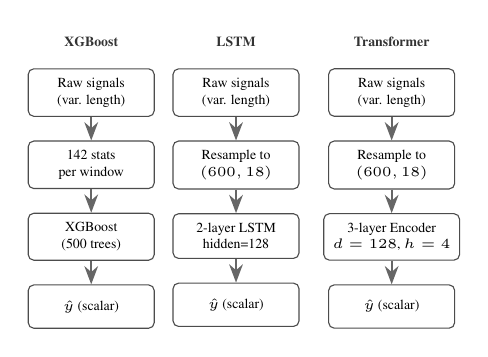
\begin{tikzpicture}[
    node distance=0.35cm and 0.2cm,
    box/.style={rectangle, rounded corners=2pt, draw=black!70,
                fill=white, align=center, font=\tiny,
                minimum height=0.55cm, minimum width=1.6cm},
    arrow/.style={->, >=Stealth, thick, draw=black!60},
    label/.style={font=\tiny\bfseries, text=black!80}
]

% XGBoost pipeline
\node[label] (xgb_title) {XGBoost};
\node[box, below=0.15cm of xgb_title] (xgb_raw) {Raw signals\\(var. length)};
\node[box, below=0.3cm of xgb_raw] (xgb_feat) {142 stats\\per window};
\node[box, below=0.3cm of xgb_feat] (xgb_model) {XGBoost\\(500 trees)};
\node[box, below=0.3cm of xgb_model] (xgb_out) {$\hat{y}$ (scalar)};
\draw[arrow] (xgb_raw) -- (xgb_feat);
\draw[arrow] (xgb_feat) -- (xgb_model);
\draw[arrow] (xgb_model) -- (xgb_out);

% LSTM pipeline
\node[label, right=1.0cm of xgb_title] (lstm_title) {LSTM};
\node[box, below=0.15cm of lstm_title] (lstm_raw) {Raw signals\\(var. length)};
\node[box, below=0.3cm of lstm_raw] (lstm_res) {Resample to\\$(600,18)$};
\node[box, below=0.3cm of lstm_res] (lstm_model) {2-layer LSTM\\hidden=128};
\node[box, below=0.3cm of lstm_model] (lstm_out) {$\hat{y}$ (scalar)};
\draw[arrow] (lstm_raw) -- (lstm_res);
\draw[arrow] (lstm_res) -- (lstm_model);
\draw[arrow] (lstm_model) -- (lstm_out);

% Transformer pipeline
\node[label, right=1.0cm of lstm_title] (tf_title) {Transformer};
\node[box, below=0.15cm of tf_title] (tf_raw) {Raw signals\\(var. length)};
\node[box, below=0.3cm of tf_raw] (tf_res) {Resample to\\$(600,18)$};
\node[box, below=0.3cm of tf_res] (tf_model) {3-layer Encoder\\$d=128$, $h=4$};
\node[box, below=0.3cm of tf_model] (tf_out) {$\hat{y}$ (scalar)};
\draw[arrow] (tf_raw) -- (tf_res);
\draw[arrow] (tf_res) -- (tf_model);
\draw[arrow] (tf_model) -- (tf_out);

\end{tikzpicture}
\caption{Three modeling pipelines from raw diagnostic signals to scalar
plasma current prediction. XGBoost compresses each window into 142
summary statistics before fitting. LSTM and Transformer both resample
signals to a fixed $(600, 18)$ time-series tensor; they differ in how
that sequence is encoded.}
\label{fig:pipeline}
\end{figure}

\subsection{Evaluation Metric}

We measure prediction quality using Normalized Root Mean Squared Error:
\begin{equation}
\text{NRMSE} = \frac{\sqrt{\frac{1}{N}\sum_{i=1}^{N}(\hat{y}_i - y_i)^2}}
{\sigma_y}
\label{eq:nrmse}
\end{equation}
where $\sigma_y$ is the standard deviation of the ground truth over the
test set. An NRMSE of 1.0 means the model is no better than predicting
the mean; values below 1.0 indicate genuine predictive
value~\cite{rousseau2026tokamark}. We compute NRMSE at the window level
and average across all test windows. This differs from TokaMark's
full shot-level hierarchical aggregation protocol~\cite{rousseau2026tokamark},
so our absolute values should not be read as direct comparisons to
TokaMark baselines.

\subsection{Robustness Score}

To enable principled comparison across architectures and scenarios, we
introduce the Robustness Score:
\begin{equation}
\text{RS} = \frac{1}{|\mathcal{S}|} \sum_{s \in \mathcal{S}}
\frac{\text{NRMSE}_\text{clean}}{\text{NRMSE}_s}
\label{eq:rs}
\end{equation}
where $\mathcal{S}$ is the full set of zero-fill corruption scenarios.
RS $= 1.0$ means corruption has no effect; values below 1.0 scale
linearly with the degree of degradation. We encourage adoption of RS
as a standard component of future plasma ML robustness evaluations.

\subsection{Corruption Scenarios}
\label{sec:scenarios}

We implement six failure scenarios, each physically grounded in real
tokamak failure modes. All scenarios are applied to the test set only;
all models are trained exclusively on clean data.

\paragraph{Scenario 1: Random dropout.}
A randomly chosen fraction $p \in \{0.10, 0.25, 0.50\}$ of all signal
values is set to zero, modeling random digitizer glitches and transient
sensor noise. The mask is applied only to positions that were already
nonzero, preserving natural acquisition gaps.

\paragraph{Scenario 2: Channel ablation.}
A randomly selected set of $n \in \{1, 3, 6\}$ complete diagnostic
channels is zeroed for the duration of the window, modeling a dead or
physically disconnected sensor.

\paragraph{Scenario 3: Per-category channel importance.}
Following the TokaMark signal taxonomy~\cite{rousseau2026tokamark}, we
zero each of eight diagnostic categories in isolation—flux loops,
pickup coils, saddle coils, Mirnov spectrograms, kinetics (interferometer
+ D-alpha), soft X-ray, active coils, and plasma current—to identify
which signals each architecture actually relies on.

\paragraph{Scenario 4: Temporal gap.}
A contiguous block covering fraction $f \in \{0.20, 0.40, 0.60\}$ of
the window is zeroed across all channels simultaneously. We test three
positions: \textit{front} (acquisition delays, consistent with our MAST
characterization), \textit{random} (mid-shot loss), and \textit{pre-event}
(the final $f$ fraction, affecting the timesteps closest to the
prediction horizon).

\paragraph{Scenario 5: Correlated diagnostic group failure.}
Motivated directly by the $r = 1.000$ NaN correlation we found in MAST
data (Section~\ref{sec:missingness}), we zero all channels belonging to
a physically related group simultaneously: kinetics (interferometer +
D-alpha), active magnetics (all pickup coil arrays), radiatives (both
soft X-ray cameras), and Mirnov spectrograms.

\paragraph{Scenario 6: Disruption-proximate failure.}
A gap of fraction $f \in \{0.10, 0.25, 0.50\}$ is injected at the very
end of the prediction window. This is the scenario with the most direct
safety implications: the sensors most critical for detecting disruption
precursors fail in the final moments before the event the model is
trying to predict.

\subsection{Mitigation Strategies}

We evaluate three imputation strategies applied after corruption, using
the corruption mask to restrict filling to artificially zeroed positions
rather than natural zeros.

\paragraph{Zero-fill.} No imputation is performed; corrupted values stay
at zero. This is the implicit behavior of TokaMark's own preprocessing
pipeline~\cite{rousseau2026tokamark} and serves as the baseline.

\paragraph{Mean-fill.} Corrupted values are replaced with the per-channel
mean from the training set.

\paragraph{Forward-fill.} The last valid observation before each gap is
carried forward until valid data resumes. This mirrors how most industrial
sensor systems behave when a reading is unavailable and is the most
physically natural strategy for a real-time control context.

\paragraph{Implementation note.} For XGBoost, temporal gap and dropout
corruption are implemented as feature-level proxies—the trajectory
statistics (first value, last value, slope) most sensitive to each gap
position are corrupted—rather than direct time-series masking used
for LSTM and Transformer. XGBoost temporal gap results are therefore
conservative estimates of the true effect.

% ─── 5. Results ──────────────────────────────────────────────────────────────
\section{Results}

\subsection{Clean-Data Baselines}

Table~\ref{tab:clean} reports clean-data NRMSE and Robustness Scores.
The Transformer achieves the best prediction accuracy on clean data
(NRMSE 0.470) but also the lowest robustness score (RS 0.765). XGBoost
sits at the other end: slightly worse clean NRMSE, highest RS (0.841).
This tradeoff—accuracy versus robustness—recurs throughout the
results and has direct architectural implications.

Our clean NRMSE values sit somewhat above the TokaMark CNN baseline of
0.429~\cite{rousseau2026tokamark}, which was trained on the full
9,270-shot dataset compared to our 200 shots. The gap is expected and
does not affect the validity of our robustness comparisons: relative
degradation patterns are determined by architecture, not by clean-data
starting point.

\begin{table}[H]
\centering
\caption{Clean-data performance and Robustness Score (RS). Lower NRMSE
is better. Higher RS indicates greater robustness.}
\label{tab:clean}
\begin{tabular}{lcc}
\toprule
Model & Clean NRMSE & RS \\
\midrule
XGBoost     & 0.494 & 0.841 \\
LSTM        & 0.496 & 0.808 \\
Transformer & 0.470 & 0.765 \\
\bottomrule
\end{tabular}
\end{table}

\subsection{Random Dropout}

Figure~\ref{fig:degradation} (left) traces NRMSE as dropout rate
increases. XGBoost degrades the most under zero-fill, reaching $+145\%$
at $50\%$ dropout—the statistical features that aggregate over the
whole window are directly disrupted when many individual values are
zeroed. LSTM and Transformer are less sensitive at $+57\%$ and $+85\%$
respectively.

Forward-fill essentially solves the dropout problem for sequence models.
At $50\%$ dropout, LSTM with forward-fill degrades by ${\sim}0\%$ and
Transformer by $-0.4\%$—both within measurement noise of their clean
baselines. The reason is straightforward: forward fill converts a
randomly damaged signal into a piecewise-constant one, and the models
have seen signals with similar step-function character in training.
XGBoost recovers only partially under mean-fill ($+39\%$ at $50\%$),
since imputing the mean into a feature vector that was computed from
corrupted values is an imperfect fix.

\subsection{Channel Ablation and Signal Importance}

Figure~\ref{fig:degradation} (center) shows overall degradation under
channel ablation, while the per-category channel importance heatmap
(Figure~\ref{fig:channel_importance})
shows a sharp hierarchy. Plasma current (\texttt{summary-ip}) is
dominant: removing it degrades LSTM by $+139.8\%$, Transformer by
$+89.1\%$, and XGBoost by $+72.7\%$. This is not surprising—plasma
current is both the primary controlled variable in a tokamak discharge
and the direct output of the task—but the magnitude of the effect
across all three architectures confirms that none of the models has
found a substitute proxy. Active coil currents are the next most
important, degrading Transformer by $+36.0\%$ and XGBoost by $+28.5\%$,
as they encode the machine's immediate control intent.

What is more interesting is what is not important. Kinetics (interferometer
+ D-alpha) and soft X-ray radiatives—the categories with the highest
natural missingness in real MAST data—cause minimal degradation when
removed (under $+20\%$ for all models). The parsimonious explanation is
that all three models have developed compensatory representations for
these signals during training, precisely because they were frequently
absent. A model that trains on 14--15\% NaN rates learns, in effect,
to treat those channels as optional.

\subsection{Temporal Gap and Disruption-Proximate Failure}

Figure~\ref{fig:proximate} isolates the three temporal gap variants and
reveals a stark asymmetry.

\paragraph{Front gap.}
Removing the first 20--60\% of the window barely affects LSTM ($+0.0\%$
at $60\%$ gap) or XGBoost ($-1.3\%$ at $60\%$ gap). This makes physical
sense: the front of a MAST shot covers the pre-plasma ramp-up, which
carries little information about the flat-top state being predicted. The
Transformer is more affected ($+52.5\%$ at $60\%$ gap), consistent with
its global attention mechanism treating all timesteps as equally
informative rather than weighting recent timesteps more heavily.

\paragraph{Proximate and pre-event failure.}
Removing the final portion of the window is catastrophic for sequence
models. LSTM hits $+212\%$ NRMSE at the first tested severity ($20\%$
gap) and stays there regardless of how large the gap grows—a hard
performance ceiling indicating that the last few timesteps are
irreplaceable for its predictions. This is the most concerning finding
in the paper: the timesteps LSTM depends on most are precisely those most
likely to be lost as a real disruption approaches. The Transformer
degrades more gradually with gap size ($+143\%$ at $20\%$, $+205\%$ at
$60\%$), suggesting its distributed attention across the full sequence
provides partial protection. XGBoost degrades moderately ($+8\%$ to
$+37\%$) because trajectory statistics like slope and last value are only
partially sensitive to end-of-window corruption.

Forward fill offers partial recovery at low proximate gap severity (LSTM
$20\%$: $+212\% \to +15\%$) but cannot recover at higher severities.
The reason is fundamental: imputing earlier values forward cannot
reconstruct the genuinely new information that the final timesteps would
have contained.

\subsection{Correlated Diagnostic Group Failure}

When entire diagnostic groups are removed simultaneously
(Figure~\ref{fig:correlated}), a different pattern emerges. LSTM
degrades most when active magnetics fail ($+26.2\%$) but is actually
less affected by kinetics failure than XGBoost—consistent with the
implicit compensation it has developed for kinetics dropouts during
training. XGBoost suffers more under kinetics ($+18.4\%$) and
radiatives ($+20.2\%$) removal, suggesting that statistical features
of those signals carry weight in its predictions that its learned
representations cannot easily replace.

Mirnov spectrogram failure causes negligible degradation in all three
models (under $+1\%$). Mirnov coils detect MHD instabilities that
typically precede locked modes and disruptions, but those instability
signatures may not be consistently present within the 150ms prediction
window in this dataset, leaving the models with little reason to rely
on them.

\subsection{Mitigation Effectiveness}

Figure~\ref{fig:mitigation} compares the three strategies across five
representative scenarios. Forward fill leads for dropout and temporal
gap, cutting LSTM $50\%$-dropout degradation from $+57\%$ to near zero
and Transformer $50\%$-dropout from $+85\%$ to near zero.

For disruption-proximate failure the picture reverses. At $50\%$
proximate gap, mean fill makes LSTM worse (NRMSE rises from $1.55$ to
$1.88$) rather than better: substituting the channel mean into the
prediction-critical final timesteps pushes the model toward an
incorrect prior exactly where it needs real signal. Forward fill
provides meaningful recovery only at the lowest severity ($10\%$
proximate gap, LSTM: $+212\% \to +1.7\%$) and loses its effectiveness
as the corrupted region grows. No simple imputation strategy resolves
the fundamental problem that the information lost during
disruption-proximate failure cannot be reconstructed from earlier
observations.

% ─── 6. Discussion ───────────────────────────────────────────────────────────
\section{Discussion}

\subsection{Architectural Inductive Bias and Robustness}

The pattern across all results can be traced to a single underlying
difference in how each model treats its input. XGBoost aggregates each
signal into a handful of statistics before making any prediction;
corrupting individual timesteps shifts those statistics by a bounded
amount and the model's predictions change proportionally. This is not
a surprising property—Chen and Guestrin~\cite{chen2016xgboost}
designed XGBoost's sparsity-aware split finding specifically to handle
missing feature values gracefully—but its implications for plasma
diagnostic robustness have not previously been demonstrated.

LSTM and Transformer both process the raw time series, and both suffer
when temporal structure is disrupted. What distinguishes them is the
nature of that disruption. The LSTM has learned, through the sequential
inductive bias of recurrent processing, to weigh the most recent
timesteps most heavily. That is normally a virtue for prediction tasks,
but here it creates a hard dependency on precisely the data that fails
first during a disruption. The Transformer's global attention distributes
sensitivity more broadly across the window, which provides some
protection against end-of-window corruption at the cost of slightly
higher sensitivity to front gaps.

\subsection{Implications for ITER-Class Devices}

The numbers in this paper should be read against a much larger backdrop.
ITER will operate in a more hostile electromagnetic and radiation
environment than any existing tokamak, including MAST~\cite{iter1999}.
Sensor failure rates will be higher, failure modes more varied, and
the cost of a missed prediction orders of magnitude greater than on a
research device. A $+212\%$ NRMSE degradation under proximate failure
does not simply mean worse prediction—it likely means the prediction
system fails the machine at the worst possible moment.

Two concrete design interventions follow from our results. First, the
pseudo-placeholder approach of Yang et al.~\cite{yang2025hl3}—training
models to explicitly distinguish missing channels from zero-valued
signal—should be standard practice rather than a device-transfer
technique. Second, the most critical signals (plasma current, active
coils) should be backed by independent redundant acquisition chains so
that a single hardware failure cannot simultaneously corrupt the signals
the model relies on most.

\subsection{Forward Fill as a Practical Recommendation}

Where architectural changes are not immediately feasible, forward fill
is a practical and well-motivated default. It is already how most
industrial sensor systems behave under failure—holding the last known
value until valid data resumes—and our results show it nearly
eliminates degradation from random dropout and mitigates low-severity
temporal gaps. Mean fill is consistently inferior and can actively
worsen performance in the disruption-proximate case by asserting a
confident but wrong prior in the most information-dense portion of the
prediction window. The practical recommendation is simple: any fusion
ML deployment pipeline should apply forward fill by default and treat
mean fill with caution.

\subsection{Reproducibility}

Every experiment in this paper can be reproduced from scratch. The
full codebase is at
\url{https://github.com/Neerav-Gupta/tokamark-robustness}, and
pre-collected data arrays (${\sim}25$~GB) with trained model checkpoints
are hosted at
\url{https://huggingface.co/datasets/Neerav-Gupta/tokamark-robustness-data}.
The underlying FAIR-MAST data is publicly accessible at
\url{https://s3.echo.stfc.ac.uk/mast/tokamark/v1}~\cite{jackson2024softwarex}.
The full experimental pipeline—data collection, training all three
models, running all corruption scenarios, and generating all six figures
—requires approximately four GPU-hours on an NVIDIA A100.

\subsection{Limitations}

\textbf{XGBoost temporal gap approximation.}
Because XGBoost operates on feature vectors rather than raw time series,
temporal gap corruption is implemented by targeting the trajectory
statistics most affected by each gap position (first value, last value,
and slope) rather than by true time-series masking. The resulting
estimates are conservative. LSTM and Transformer temporal gap results
use exact masking.

\textbf{Training set size.}
All three models train on 200 shots, compared to TokaMark's full
9,270-shot training set. This constrains clean-data accuracy but does
not affect the relative degradation patterns, which are determined by
architecture rather than training set size.

\textbf{Single task.}
We evaluate Task~4-4 only. Robustness behavior on other TokaMark tasks
—particularly the binary disruption classification tasks in Group~4—
may differ and warrants separate study.

\textbf{Single training run.}
Each model is trained once. Run-to-run variance is not characterized,
and results should be interpreted with that caveat when making direct
performance comparisons.

% ─── 7. Conclusion ───────────────────────────────────────────────────────────
\section{Conclusion}

We have built and evaluated the first systematic robustness benchmark for
plasma diagnostic ML models under realistic sensor failure conditions.
Three findings stand out as both robust and actionable. Disruption-proximate
sensor failure is catastrophic for LSTM models, producing a $+212\%$ NRMSE
increase that does not diminish as the corrupted region grows—a direct
consequence of the architecture's learned dependence on final-window
timesteps. Forward-fill imputation resolves the random dropout problem
for sequence models almost entirely, at zero architectural cost. Plasma
current is the critical signal: remove it, and all three architectures
degrade sharply regardless of what else is intact.

The deeper message is architectural. An LSTM trained to lean on the most
recent observations is well-suited for smooth prediction tasks but poorly
suited for disruption prediction, where the sensor environment is most
degraded at the very moment the model needs to perform. Building fault
tolerance into plasma prediction systems—whether through explicit
missing-data handling, architectural choices, or sensor redundancy design
—is not an implementation detail but a prerequisite for safe deployment
on ITER-class devices. We hope the Robustness Score and the benchmark
methodology introduced here provide a foundation for that work.

\section*{Acknowledgements}

The author thanks the TokaMark team at UKAEA, IBM Research Europe, and
STFC Hartree Centre for releasing TokaMark, TokaMind, and the FAIR-MAST
dataset as open resources, making this work possible.

% ─── References ──────────────────────────────────────────────────────────────
\renewcommand{\bibfont}{\footnotesize}
\setlength{\bibsep}{2pt}
\bibliographystyle{unsrtnat}
\bibliography{references}

% ─── Appendix: Figures ───────────────────────────────────────────────────────
\clearpage
\onecolumn
\appendix
\section*{Figures}

\begin{figure*}[h]
\centering
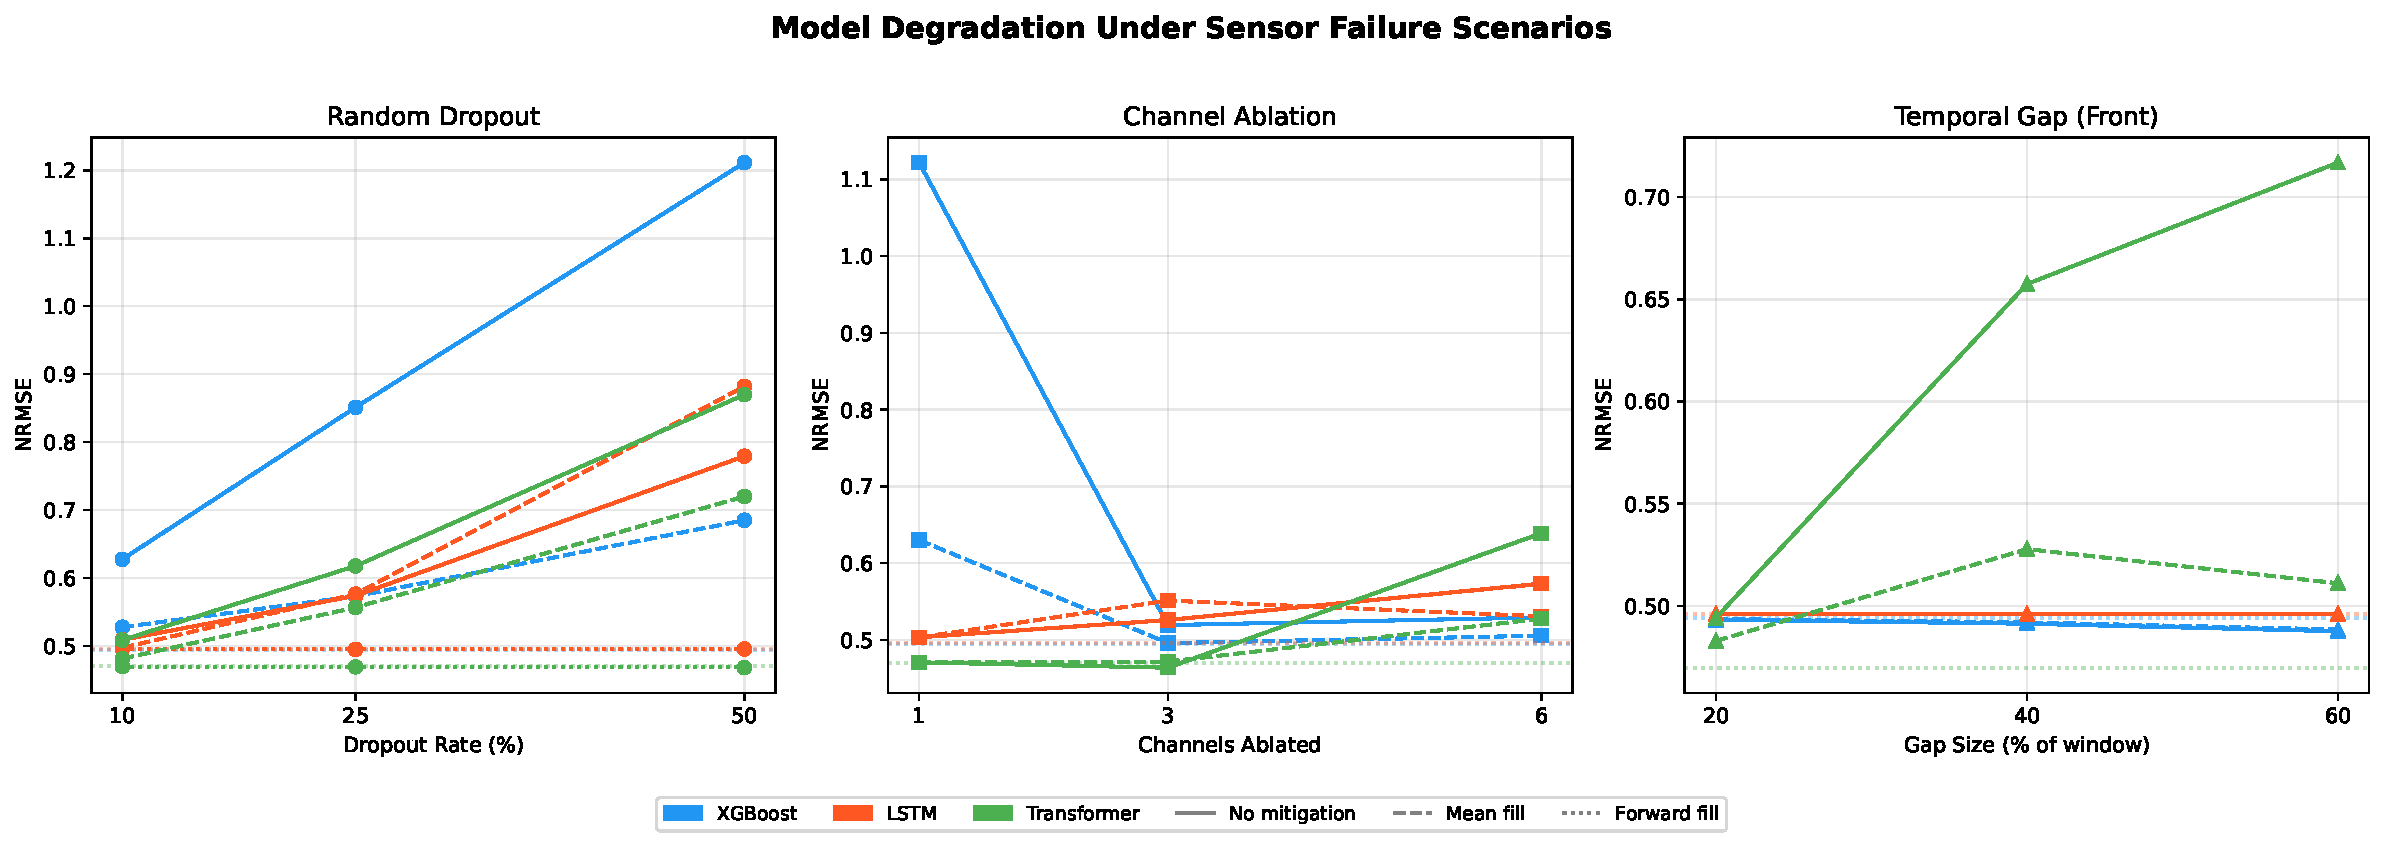
\includegraphics[width=\textwidth]{../plots/fig1_degradation_curves.pdf}
\caption{NRMSE under three corruption scenarios across severity levels.
Dotted horizontal lines show each model's clean baseline. Solid lines
show zero-fill (no mitigation); dashed lines show mean-fill; dotted
lines show forward-fill. \textbf{Left:} Random dropout—XGBoost
degrades most severely but forward fill nearly eliminates degradation
for LSTM and Transformer. \textbf{Center:} Channel ablation—LSTM
and Transformer show consistent degradation; XGBoost shows high
variance due to random channel selection. \textbf{Right:} Temporal
gap (front position)—LSTM and XGBoost are nearly unaffected;
Transformer degrades moderately at large gap sizes.}
\label{fig:degradation}
\end{figure*}

\begin{figure*}[h]
\centering
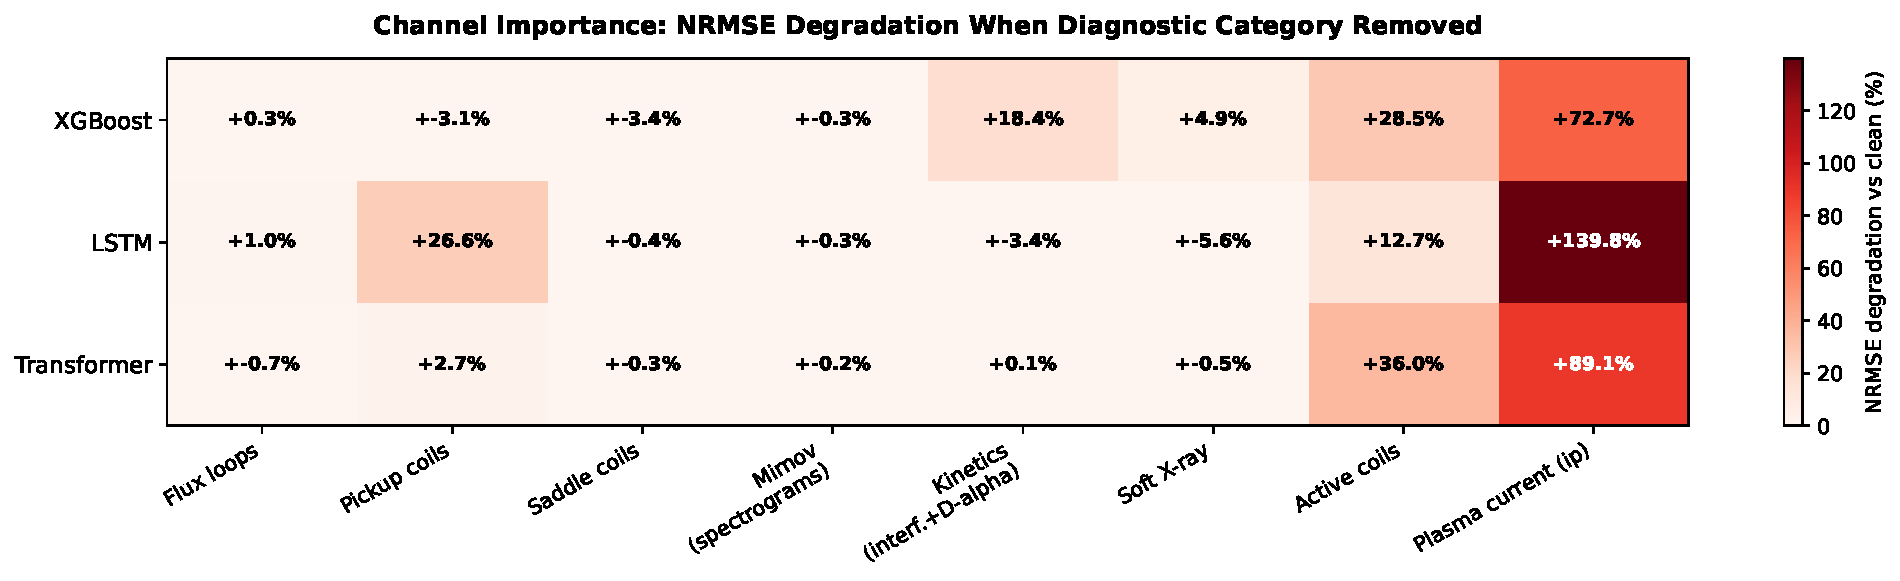
\includegraphics[width=\textwidth]{../plots/fig2_channel_importance.pdf}
\caption{Per-category channel importance heatmap. Values show NRMSE
degradation (\%) when each diagnostic category is completely removed.
Plasma current dominates across all architectures. Active coils are
the second most critical category. Kinetics and radiatives—despite
having the highest natural missingness rates—cause minimal degradation,
suggesting implicit robustness learned from training data.}
\label{fig:channel_importance}
\end{figure*}

\begin{figure*}[h]
\centering
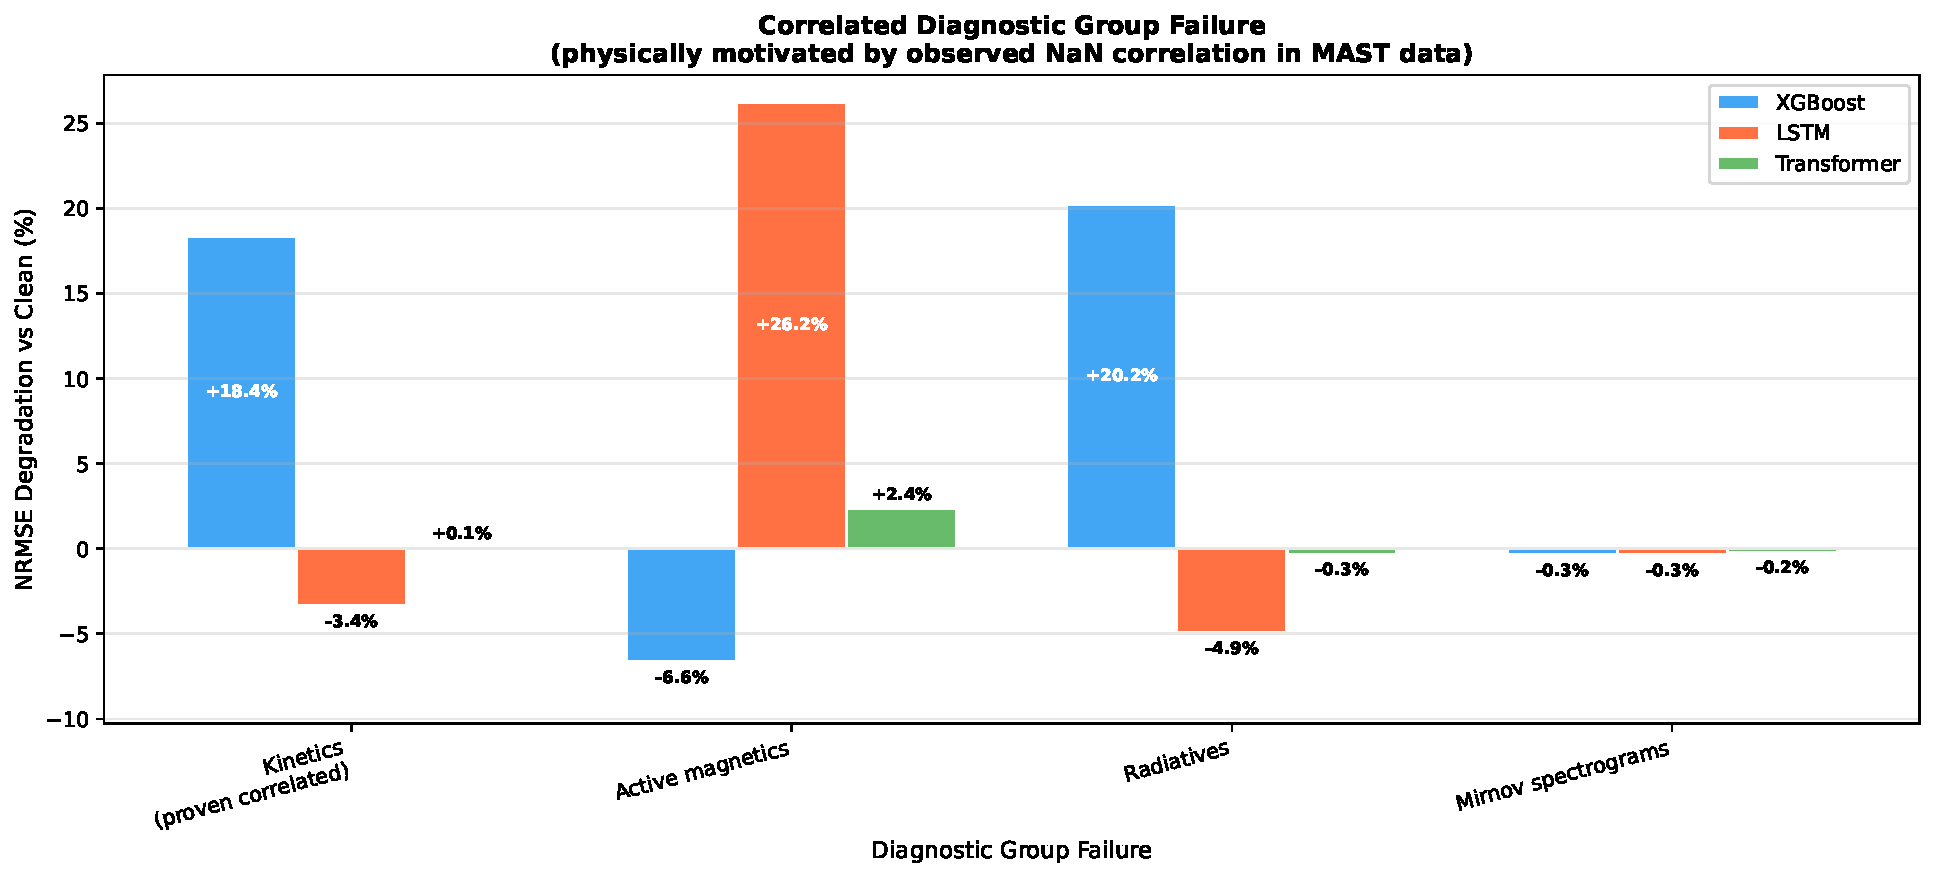
\includegraphics[width=\textwidth]{../plots/fig3_correlated_failure.pdf}
\caption{NRMSE degradation (\%) under correlated diagnostic group
failure—simultaneous zeroing of all signals within a physically
related group. Group definitions are empirically motivated by the
observed NaN correlation structure in MAST data
(Section~\ref{sec:missingness}). Negative values indicate slight
NRMSE improvement, likely from removal of noisy signals that
contributed adversarial gradients during prediction.}
\label{fig:correlated}
\end{figure*}

\begin{figure*}[h]
\centering
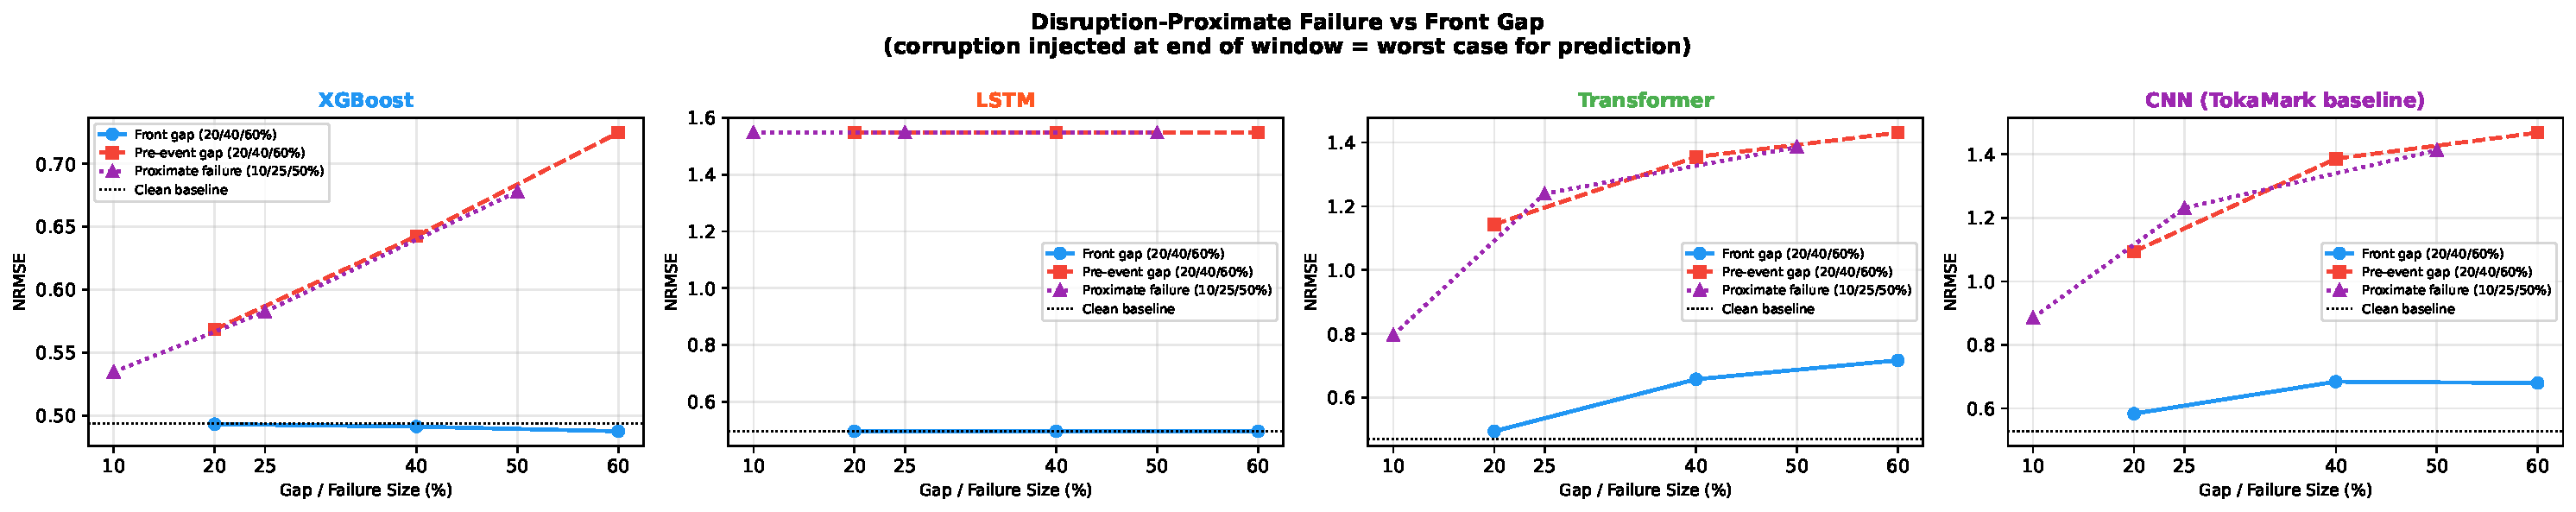
\includegraphics[width=\textwidth]{../plots/fig4_proximate_comparison.pdf}
\caption{Comparison of front gap, pre-event gap, and
disruption-proximate failure. Front gap (blue circles) causes
negligible degradation for LSTM and XGBoost but moderate degradation
for the Transformer. Pre-event gap (red squares) and proximate failure
(purple triangles) cause catastrophic, severity-independent degradation
in LSTM—indicating a reliance on the final timesteps that is a
fundamental architectural vulnerability for disruption prediction.
Transformer degrades more gradually. XGBoost remains comparatively
robust.}
\label{fig:proximate}
\end{figure*}

\begin{figure*}[h]
\centering
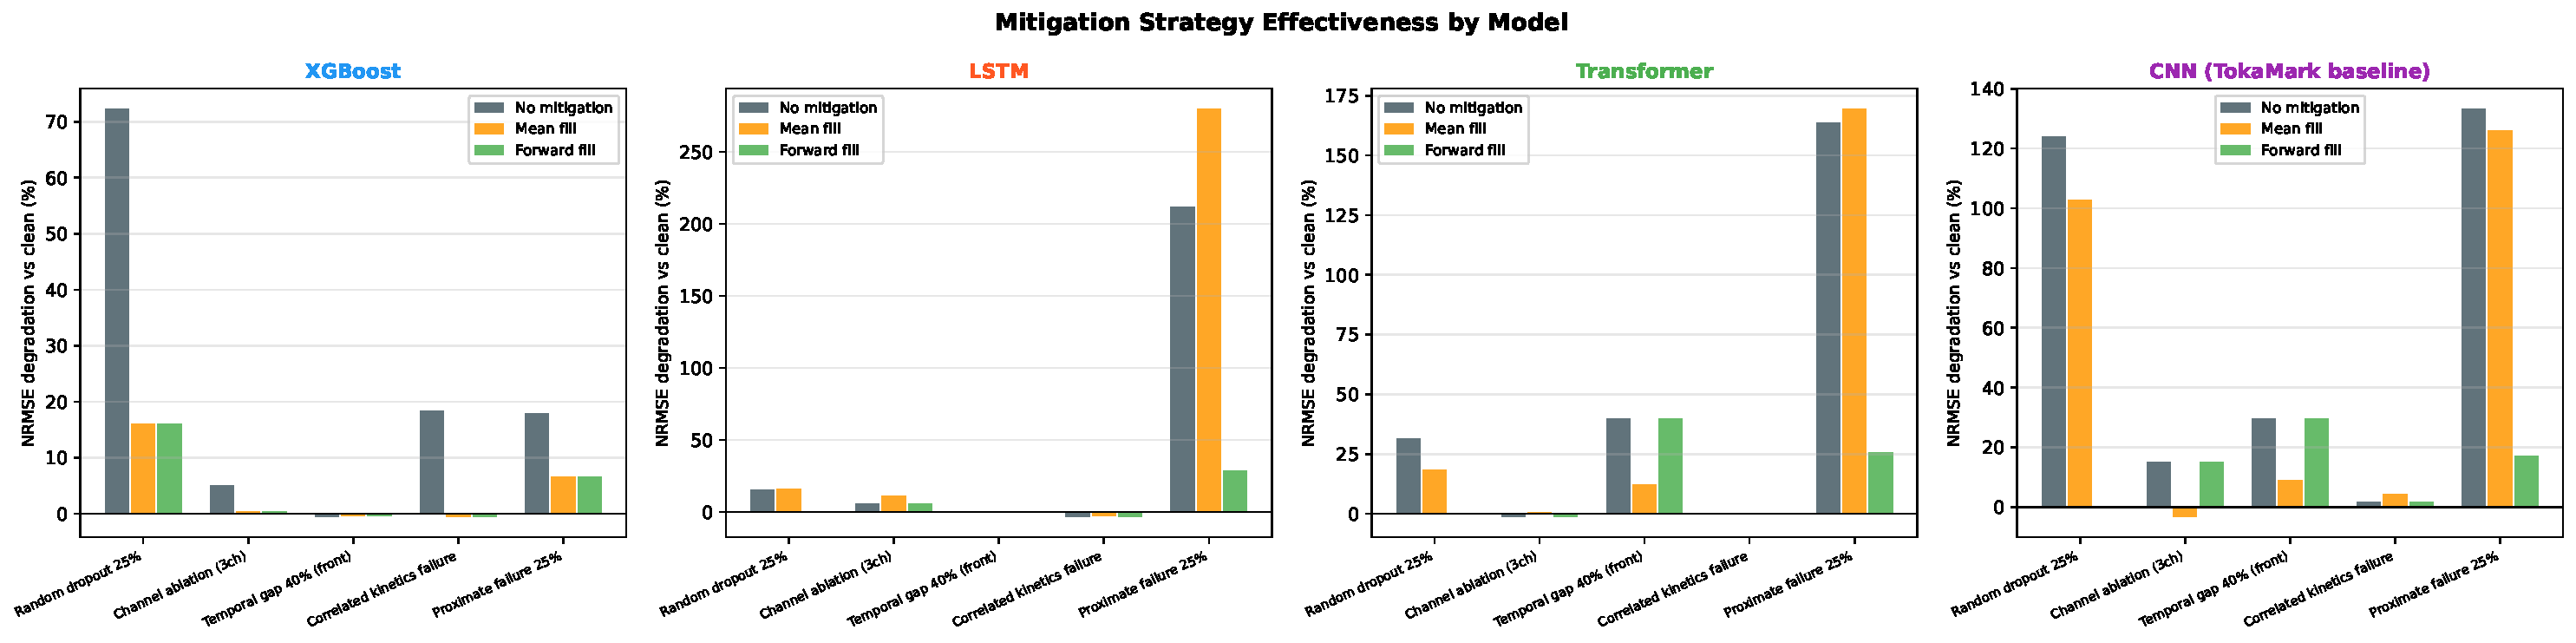
\includegraphics[width=\textwidth]{../plots/fig5_mitigation_effectiveness.pdf}
\caption{Mitigation strategy effectiveness across five representative
scenarios. Forward fill (green) is consistently most effective for
dropout and temporal gap scenarios, reducing degradation to near zero
for sequence models under random dropout. Mean fill (orange) provides
partial recovery for XGBoost. Neither strategy effectively mitigates
disruption-proximate failure at high severity—highlighting the
fundamental limitation of simple imputation for end-of-window
corruption.}
\label{fig:mitigation}
\end{figure*}

\begin{figure*}[h]
\centering
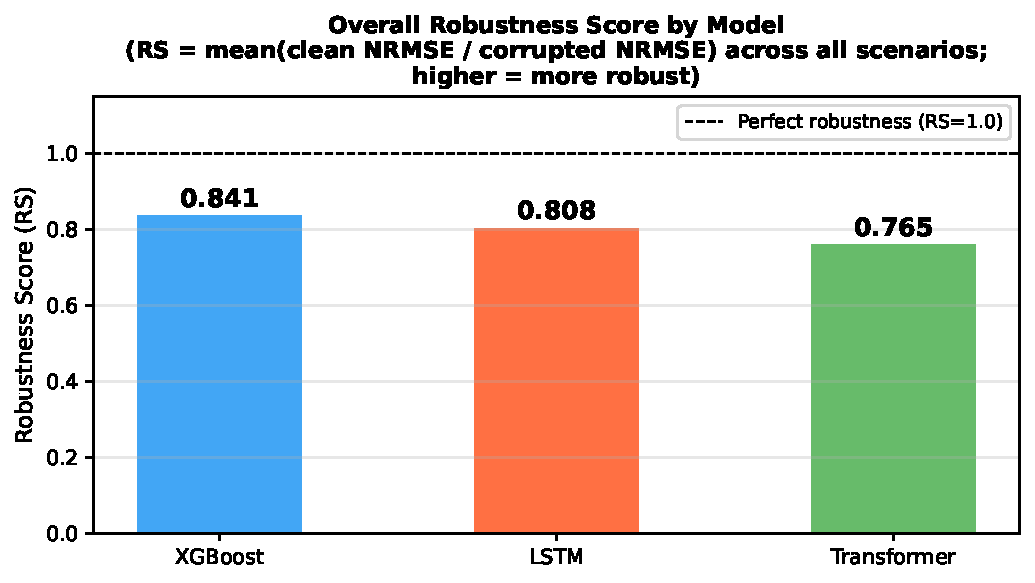
\includegraphics[width=0.5\textwidth]{../plots/fig6_robustness_scores.pdf}
\caption{Overall Robustness Score (RS) by model. RS $= 1.0$ indicates
perfect robustness; lower values indicate greater degradation. XGBoost
achieves the highest RS (0.841), reflecting the inherent robustness
of statistical feature aggregation to individual value corruption. The
Transformer achieves the best clean accuracy but the lowest RS (0.765),
revealing a tradeoff between predictive performance and fault tolerance
that has direct implications for deployment in safety-critical systems.}
\label{fig:robustness}
\end{figure*}

\end{document}